\documentclass[border=4pt]{standalone}
\usepackage{tikz}
\usetikzlibrary{arrows.meta,positioning}
\tikzset{state/.style={circle,draw,minimum size=11mm,inner sep=1pt}}
\begin{document}
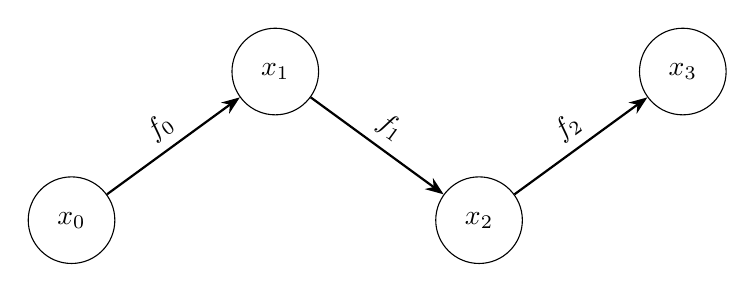
\begin{tikzpicture}[node distance=11mm and 18mm,>=Stealth]
  \node[state] (x0) {$x_0$};
  \node[state,above right=of x0] (x1) {$x_1$};
  \node[state,below right=of x1] (x2) {$x_2$};
  \node[state,above right=of x2] (x3) {$x_3$};
  \draw[->,thick] (x0) -- node[above,sloped] {$f_0$} (x1);
  \draw[->,thick] (x1) -- node[above,sloped] {$f_1$} (x2);
  \draw[->,thick] (x2) -- node[above,sloped] {$f_2$} (x3);
\end{tikzpicture}
\end{document}
